\documentclass[article, backcover, french, nodocumentinfo]{upmethodology-document}
% Encoding
	\usepackage[utf8]{inputenc}
	%\usepackage[latin1]{inputenc}
	\usepackage[T1]{fontenc}

% Language
	%\usepackage[francais,english]{babel} % Second language = main language

% Show a summary of the layout of the current document with \layout.
	%\usepackage{layout}

% For easy management of document margins and the document page size.
	%\usepackage[top=2cm, bottom=1.8cm, left=1.8cm, right=1.8cm, head=14pt, foot=36pt]{geometry}

% Lets you change line spacing.
	%\usepackage{setspace}

% Euro symbol
	%\usepackage{eurosym}

% Fonts (include only one)
	%\usepackage{bookman}
	%\usepackage{charter}
	%\usepackage{newcent}
	\usepackage{lmodern}
	%\usepackage{mathpazo}
	%\usepackage{mathptmx}

% Enables typesetting of hyperlinks
	%\usepackage{url}
	\usepackage{hyperref}

% Verbatim environment
	%\usepackage{verbatim}
	%\usepackage{moreverb}
	\usepackage{fancyvrb}

% Code listing
	\usepackage{listings}

% To change header and footer of any page of the document.
	\usepackage{fancyhdr}

% Allows you to insert graphic files within a document.
	%\usepackage{graphicx}

% Allows figures or tables to have text wrapped around them.
	%\usepackage{wrapfig}

% Adds support for colored text.
	\usepackage{xcolor}

% Allows tables rows and columns to be colored, and even individual cells.
	%\usepackage{colortbl}

% Mathematics
	\usepackage{amsmath}
	\usepackage{amssymb}
	\usepackage{mathrsfs}
	%\usepackage{asmthm}
	%\usepackage{mathtools}
	%\usepackage{bm} % Greek letters in math mode

% Provides control over the layout of the three basic list environments: enumerate, itemize and description.
	%\usepackage{enumitem}

% Interface to sectioning commands for selection from various title styles
	%\usepackage[nobottomtitles]{titlesec}

% Highly customized stacking of objects, insets, baseline changes, etc.
	\usepackage{stackengine}

% Routines for constrained scaling and stretching of objects, relative to a reference object or in absolute terms
	\usepackage{scalerel}

% Provides control over the typography of the Table of Contents, List of Figures and List of Tables, and the ability to create new ‘List of ...’.
	%\usepackage{tocloft}
	%\usepackage{titletoc}

% Advanced bibliography handling.
	%\usepackage{bibtex}
	%\usepackage{biblatex}

% Allows customization of appearance and placement of captions for figures, tables, etc.
	%\usepackage{caption}

% Provides the multicols environment which typesets text into multiple columns.
	%\usepackage{multicol}

% This package simplifies the insertion of external multi-page PDF or PS documents.
	%\usepackage{pdfpages}

% Prints out all index entries in the left margin of the text.
	%\usepackage{showidx}

% It allows to define multiple floats (figures, tables) within one environment giving individual captions and labels in the form 1a, 1b.
	%\usepackage{subcaption}

% Lets you insert notes of stuff to do with the syntax \todo{Add details.}.
	%\usepackage{todonotes}

% Text Companion fonts, which provide many text symbols (such as baht, bullet, copyright, musicalnote, onequarter, section, and yen), in the TS1 encoding.
	\usepackage{textcomp}

% For floating elements placement
	\usepackage{float}

% Personnal packages
	\usepackage{packages/MagicListings}
	\usepackage{packages/AlgorithmDefinition}

% For more information about UPmethodology: https://www.ctan.org/pkg/upmethodology

%=======================================================================================================
%=============================================== Informations ==========================================
%=======================================================================================================

%%% Document Information and Declaration
\declaredocument{Jeu tactique: Pogo}{Projet d'IA41}{UTBM\_IA41\_Pogo\_P17}

%%% Abstract and Key-words
\setdocabstract[french]{Projet UTBM de l'UV IA41 du semestre de printemps 2017}
\setdockeywords[french]{UTBM, IA41, Pogo}

%%% Document Authors and Validators
\addauthorvalidator*[julien.barbier@utbm.fr]{Julien}{Barbier}{Étudiant en INFO02}
\addauthorvalidator*[kadir.ercin@utbm.fr]{Kadir}{Ercin}{Étudiant en INFO02}
\addauthorvalidator*[maxime.pinard@utbm.fr]{Maxime}{Pinard}{Étudiant en INFO02}

%%% Informed People
\addinformed*[fabrice.lauri@utbm.fr]{Fabrice}{Lauri}{Professeur de l'UV IA41}

%%% Copyright and Publication Information
\setcopyrighter{Julien Barbier, Kadir Ercin et Maxime Pinard}
\setpublisher{Julien Barbier, Kadir Ercin et Maxime Pinard}
\setprintingaddress{France}

%%% Version
\incversion{\makedate{\the\day}{\the\month}{\the\year}}{Initial version.}{\upmpublic}

%=======================================================================================================
%================================================== Configs ============================================
%=======================================================================================================

% Change Front Page Layout
%\setfrontcover{modern} % modern or classic

% Change Illustration Picture
%\setfrontillustration[1.3]{figures/figure}

% Source code formatting
\upmcodelang{cpp} % uml, java or cpp

% Prevent page breaks in paragraphs
\predisplaypenalty=1000
\postdisplaypenalty=1000
\clubpenalty=1000

% Minimal space required in the bottom margin not to move the title on the next page
%\renewcommand{\bottomtitlespace}{.1\textheight}

% Links config, especialy for the table of contents
\hypersetup{
    colorlinks=true,
    linkcolor=black,
    urlcolor=blue,
    linktoc=all
}

% French language config
%\frenchbsetup{StandardLayout=true,ReduceListSpacing=false,CompactItemize=false}

%=======================================================================================================
%================================================= Functions ===========================================
%=======================================================================================================

%Paragraph with line break
\newcommand{\p}[1]{\paragraph{#1\\}}

% Function to print a warning sign
\newcommand{\dangersign}[1][2.5ex]
	{\renewcommand{\stacktype}{L}
		{\scaleto{\stackon[1pt]{\color{red}$\triangle$}{\fontsize{4pt}{4pt}\selectfont !}}{#1}}}

% Definition of some dt/dx/dy shortcuts for integrals
\newcommand{\dt}
{\;\mathrm{d}\,t}

\newcommand{\dx}
{\;\mathrm{d}\,x}

\newcommand{\dy}
{\;\mathrm{d}\,y}

% Definition of \Witem for 'itemize' environment with a warning sign
\newcommand{\Witem}
{\item[\dangersign{}]}

% Definition of a Max function shortcut
\newcommand{\Max}[2][ ]
{\underset{#1}{\text{Max}}\,#2}

% Definition of a Min function shortcut
\newcommand{\Min}[2][ ]
{\underset{#1}{\text{Min}}\,#2}


\begin{document}
	\upmdocumentsummary{}
	\upmdocumentauthors{}
	%\upmdocumentvalidators{}
	\upmdocumentinformedpeople{}
	\upmpublicationpage{}
	\thispagestyle{empty}
	\tableofcontents{}
	\lstlistoflistings{}
	\listoffigures{}
	\newpage{}

	\section{Sujet, règles du jeu}
		\subsection{Présentation}
			Le but de ce projet est de réaliser une IA capable de jouer au jeu de Pogo. Pour cela l'algorithme \textbf{MinMax} et son optimisation \textbf{AlphaBeta} seront utilisés. Il doit aussi être possible de tester l'IA. Le langage utilisé pour réaliser le projet est le C++ norme 2011.
		\subsection{Règles}
		\subsection{Objectifs}
			\p{Objectif premiers}
				Il faut réaliser une IA mais il faut aussi pouvoir tester cette dernière pour évaluer sa performance. Pour pouvoir tester l'IA il faut que le programme propose de jouer en Humains contre IA mais aussi en IA contre IA. Pour cela nous avons fixé les objectif suivants:
				\begin{itemize}
					\item Implémenter la logique d'un jeu de Pogo
					\item Réaliser une IA capable de jouer au jeu
					\item Réaliser une interface homme-machine pour permettre a l'utilisateur de visualiser le jeu et d'y jouer
				\end{itemize}
			\p{Objectif supplémentaires}
				Nous avons rajouter quelques objectifs supplémentaires afin d'améliorer le programme, faciliter les test de l'IA et élargir les possibilités de modification de l'IA.
				\begin{itemize}
					\item Permettre de jouer en Humain contre Humain
					\item Permettre de choisir la profondeur d'exploration de l'arbre de l'IA
					\item Proposer plusieurs fonctions d'évaluation d'une situation de jeu et un comparatif de ces dernières
					\item \color{green} Ajouter une non-IA (mouvements aléatoires)
				\end{itemize}
		\subsection{Notes}
			\p{Détails}
				Les fonctions importantes et liées a l'IA seront expliqué et leur fonctionnement détaillé (souvent par un algorithme). Pour les autres fonction se référer a la documentation Doxygen du code.
				\begin{upminfo}
					Doxygen est un générateur de documentation sous licence libre, une documentation web peut être généré, pour cela voir \href{http://www.stack.nl/~dimitri/doxygen/}{le site web de Doxygen}.
				\end{upminfo}
			\p{Diagrammes}
				Les diagrammes utilisé pour expliciter les classes sont des diagrammes de classe UML dont les spécification peuvent etre obtenues sur le site \href{http://www.omg.org/spec/UML/}{Object Management Group}
	\section{Réalisation}
		\subsection{Représentation du jeu}
			\subsubsection{pions}
			\subsubsection{Piles de pions}
			\subsubsection{Plateau}
		\subsection{Structure de l'IA}
			\subsubsection{MinMax}
				\lstinputalgo[caption=MinMax]{algorithms/MinMax.algo}
			\subsubsection{AlphaBeta}
			\subsubsection{Génération des coups}
			\subsubsection{Fonction d'évaluation}
				\paragraph{}
					Afin d'évaluer le partie nous comptons pour un joueur  le nombre de piles qu’il contrôle, que nous divisons par le nombre total de piles présentes sur le jeu. Notre évaluation représente donc le pourcentage de piles que nous contrôlons. Eval = 0 représente donc une défaite pour le joueur qui évalue car il ne possède aucune pile et Eval = 1 une victoire car il les contrôle toutes. On a donc $Eval \in [0,1]$.\\
					De façon formelle :
					\[
					x_{i} = \left\{
					\begin{array}{ll}
						1 \mbox{ si  on contrôle la pile de la case i} \\
						0  \mbox{ sinon}
					\end{array}
					\right.
					\]
					et $n$ le nombre de piles présentes sur le plateau
					\[Eval = \frac{1}{n}  \sum_{i = 1}^{9} x_{i}\]
					Exemple:
					\begin{center}
						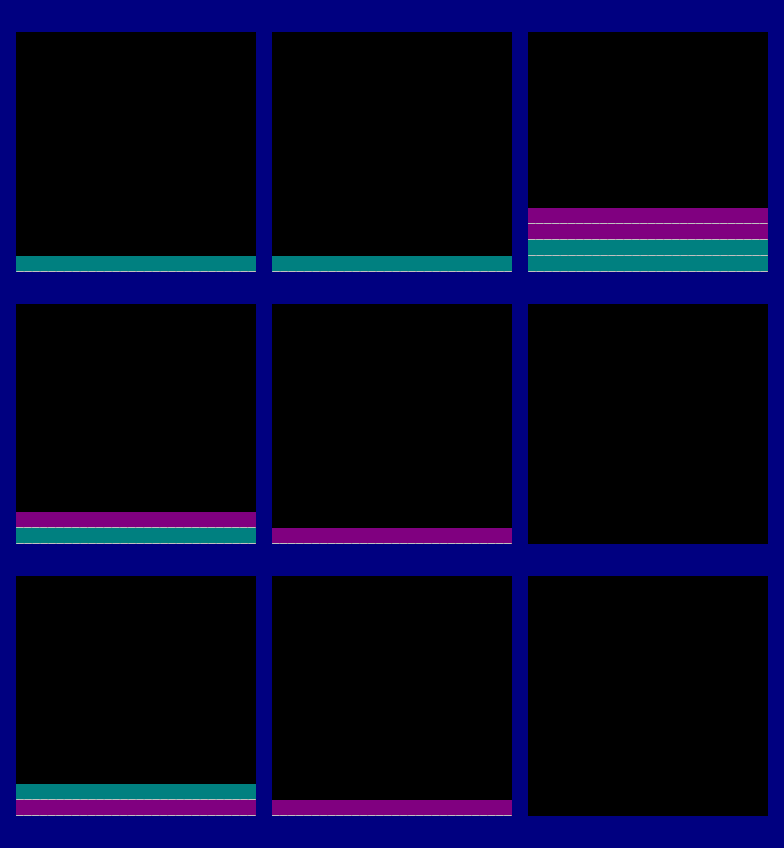
\includegraphics[width=0.6\textwidth]{figures/Eval.png}
					\end{center}
				\paragraph{}
					Dans ce cas pour le joueur violet contrôle 4 piles, et le nombre de piles sur le plateau est de 7, ce qui nous donne $Eval = \frac{4}{7} \simeq 0,571$
		\subsection{Interface utilisateur}
			\subsubsection{Fonctionnalités}
				L'interface graphique est entièrement réalisée en console avec un style ``graphique''. Il y a deux interfaces principales, les menu et messages (d'information, d'erreur\ldots) et le plateau du jeu de Pogo.
				\p{Menus}
					Avant de commencer une partie plusieurs menus se suivent:
					\begin{itemize}
						\item Menus principal: choix du mode de jeu
							\begin{itemize}
								\item Humain contre Humain
								\item Humain contre IA
								\item IA contre IA
							\end{itemize}
						\item Si jeu avec IA (une ou deux): Menu de choix de la profondeur d'exploration de l'arbre de/des IA
						\item Menu de choix de l'ordre de jeu
					\end{itemize}
				\p{Plateau de jeu}
					Le plateau de jeu en 3 $\times$ 3 fait une taille de 98 caractères de large et 53 caractères de haut, si la console n'est pas suffisamment grande pour afficher le plateau un message demandant d'agrandir la console apparaitra. Dans le cas d'une utilisation sous Windows si l'écran ne permet pas d'étendre suffisamment la console on peut faire:\\
					\textit{clique droit sur la barre supérieure > Propriétés > Police > Taille}\\
					et réduire la taille de la police pour augmenter la largeur et hauteur en caractères de la console et permettre l'affichage du plateau.\\

					Lors du tour d'un joueur humain, le plateau permet de choisir un mouvement de la façon suivante:
					\begin{itemize}
						\item Choix de la pile de départ
						\item Choix du nombre de pions a prendre
						\item Choix de la pile d'arrivé
					\end{itemize}
					Lors du choix de la pile de départ et d'arrivé, les choix valides serons affichés en vert.
			\subsubsection{Utilisation}
				\p{Menus}
					Les menus simples s'utilisent avec les contrôles suivants:
					\begin{description}
						\item[Page précédente] Premier choix
						\item[Page suivante] Dernier choix
						\item[Flèche du haut] Choix précédent
						\item[Flèche du bas] Choix suivant
						\item[Entré] Valider le choix
						\item[Échap] Quitter (pas toujours possible)
					\end{description}
					Les menus a options s'utilisent avec les contrôles des menus simples avec en plus que les contrôles suivants:
					\begin{description}
						\item[Début] Première valeur de l'option
						\item[Fin] Dernière valeur de l'option
						\item[Flèche de gauche] Valeur précédente de l'option
						\item[Flèche de droite] Valeur suivante de l'option
					\end{description}
				\p{Plateau de jeu}
					Lors de la sélection d'une pile, les contrôles suivants sont utilisables:
					\begin{description}
						\item[Flèche du haut] Bouger la sélection en haut
						\item[Flèche du bas] Bouger la sélection en bas
						\item[Flèche de gauche] Bouger la sélection a gauche
						\item[Flèche de droite] Bouger la sélection a droite
						\item[Entré] Valider le choix
						\item[Échap] Quitter la partie
					\end{description}
					Lors de la sélection du nombre de pions a prendre dans une pile:
					\begin{description}
						\item[Flèche du haut] Diminuer le nombre de pions pris
						\item[Flèche du bas] Augmenter le nombre de pions pris
						\item[Entré] Valider le choix
						\item[Échap] Quitter la partie
					\end{description}
			\subsubsection{Réalisation}
				\begin{figure}[h!]
					\centering
					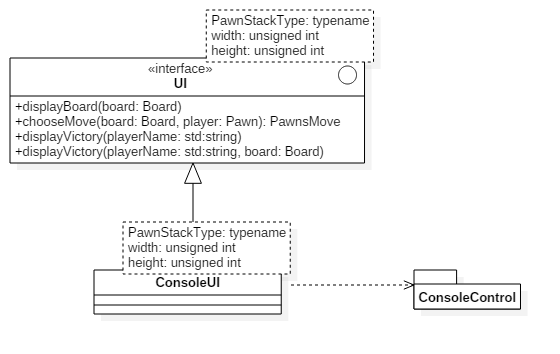
\includegraphics[width=0.7\textwidth]{figures/UIDiagram}
					\caption{UI et ConsoleUI: diagramme de classe}
					\label{fig:UIDiagram}
				\end{figure}
				L'interface utilisateur du projet est constitué de deux classes:
				\p{UI}
					\texttt{UI} est l'interface (classe purement abstraite) a implémenter pour réaliser une interface homme machine utilisable dans le projet. Elle a 3 paramètres de template: le type de stack utilisé, la largeur du plateau et sa hauteur. Elle possèdes des fonctions pour afficher le plateau et la victoire mais aussi pour permettre au joueur humain de choisir un mouvement.
				\p{ConsoleUI}
					\texttt{ConsoleUI} est l'implémentation qu'utilise le projet, elle est entièrement en console mais emprunte beaucoup aux interface graphiques, elle a été réalisée avec la librairie C, compatible C++ \textbf{ConcoleControl} développée par Maxime Pinard, membre du groupe du projet. Le projet utilise la version 0.2 de la librairie.
					\begin{figure}[h!]
						\centering
						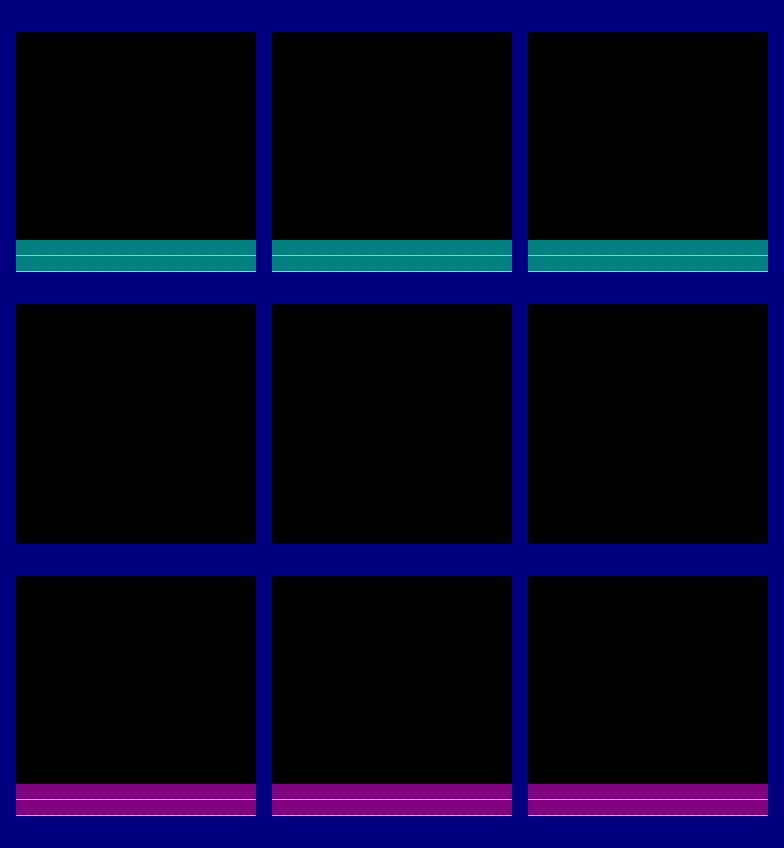
\includegraphics[width=0.7\textwidth]{figures/ConsoleUI}
						\caption{ConsoleUI: affichage en console du plateau de jeu}
						\label{fig:ConsoleUI}
					\end{figure}
				\p{ConcoleControl}
					Fonctionnalités:
					\begin{itemize}
						\item Obtention d'informations sur la console (largeur, hauteur\ldots)
						\item Positionnement du curseur
						\item Changement des couleurs d'arrière plan et de premier plan
						\item Gestion des inputs
						\item Dessin géométrique (lignes, rectangle)
						\item Interface utilisateur:
							\begin{itemize}
								\item Menu
								\item Menu d'options
								\item Messages
							\end{itemize}
						\item \ldots
					\end{itemize}
					Avantages:
					\begin{itemize}
						\item Multiplateforme
						\item Pas de dépendances
						\item Utilisé en sous module compilé en même temps que le projet
					\end{itemize}
					Pour plus d'informations, voir \href{https://github.com/pinam45/ConsoleControl}{la page Github de la librairie}.
				\p{Résultat}
					L'interface du jeu est multiplateforme, dessinée en console, principalement en couleur mais aussi avec des caractères. Nous avons choisit des couleur différente du jeu original de Pogo pour plus de lisibilité dans la console mais les couleurs et les caractères utilisés sont tous des champs privés de \textit{ConsoleUI} et sont donc configurables dans le fichier \texttt{ConsoleUI.hpp}.
	\section{Compilation}
		\subsection{Informations}
		\subsection{Make}
		\subsection{CMake}
	\section{Résultats}
		\subsection{IA contre IA}
		\subsection{IA contre Humain}
%\begin{upmcaution}
%	This is an example of a caution message. This text must be rendered with enough height (usually 2 lines of text) to avoid intersection between the caution icon and the box frame.
%\end{upmcaution}
%\begin{upminfo}
%	This is an example of an information message. This text must be rendered with enough height (usually 2 lines of text) to avoid intersection between the caution icon and the box frame.
%\end{upminfo}
%\begin{upmquestion}
%	This is an example of a question message. This text must be rendered with enough height (usually 2 lines of text) to avoid intersection between the caution icon and the box frame.
%\end{upmquestion}
%\begin{figure}[h!]
%	\centering
%	\includegraphics[width=0.5\textwidth]{figures/sample} % or <figures/sample.jpg>
%	\caption{sample figure}
%	\label{fig:sampleFigure}
%\end{figure}
\end{document}
